\chapter{Einführung}

In modernen Videospielen werden verschiedenste Effekte verwendet um dem Spieler die Welt glaubhafter und realer wirken zu lassen.
Einer davon ist die Zerstörung von unterschiedlichen Objekten im Spiel wie einfache Gegenstände oder in manchen Spielen sogar zerstörbare Landschaften.
Aufgrund des hohen Rechenaufwands wird in Spielen jedoch meist ein statischer Ansatz für solch destruktive Objekte verwendet, das heißt ein Model wird von einem Artist 
bereits vorher fragmentiert modelliert und zum gewünschten Zeitpunkt im Spiel einfach ausgetauscht. Dieser Ansatz hat jedoch auch Nachteile. 
Zum Beispiel wird die Entwicklungszeit eines Spieles verlängert, da der Artist 3D-Modelle mit unterschiedlichen Frakturierungen erstellen muss,
und zusätzlich kann es sein, dass die Spielerinteraktion in der Spielumgebung durch vorgebrochene Objekte einteschränkt wird \cite{Najim.DynamicFracturing}.

Durch bisherige Bemühungen auf diesem Gebiet konnte Algorithmen entwickelt werden, welche in Echtzeit ausgeführt werden können und dadurch
einen dynamischeren Effekt erzielen. Diese Algorithmen zur Erstellung von Fragmentierungen basieren beispielsweise auf dem Voronoi Diagramm
oder der Finite-Elemente-Methode \cite{Parker.Real-TimeDeformation}.


\section{Voronoi Diagramm}

Ausgehend von einer endlichen Menge an verschiedenen, isolierten Punkten in einem Raum, werden alle Orte mit dem nächstgelegenen Punkt der Punktmenge assoziiert.
Das Ergebnis ist eine Unterteilung des Raumes in eine Menge von Regionen, die sogenannten Voronoi Zellen, die zusammen das Voronoi Diagramm bilden, 
wie in Abbildung \ref{fig:voronoi1} zu sehen ist \cite{Okabe.SpatialTessellationsVoronoi}.



\begin{figure}[H]
    \centering
    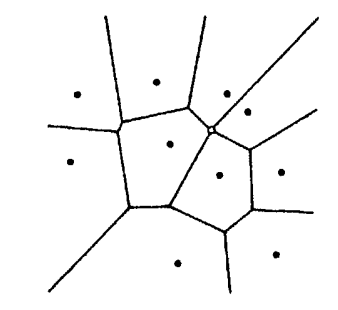
\includegraphics[width=0.35\linewidth]{PICs/voronoi.PNG}
    \caption{Voronoi Diagramm \protect\cite{Okabe.SpatialTessellationsVoronoi}}
    \label{fig:voronoi1}
\end{figure}

Diese Voronoi Zellen werden als Primitive genutzt, um zerstörbare 3D Regionen zu repräsentieren, können schnell und einfach berechnet werden und auf praktisch alle 3D-Modelle
angewendet werden \cite{Najim.DynamicFracturing}.

genralized in a variety of ways (chapter 3 in okabe)
data structures to represent voronoi (chapter 4)



\section{Finite Element Methode}
